
\begin{figure}[t]
  \begin{center}
    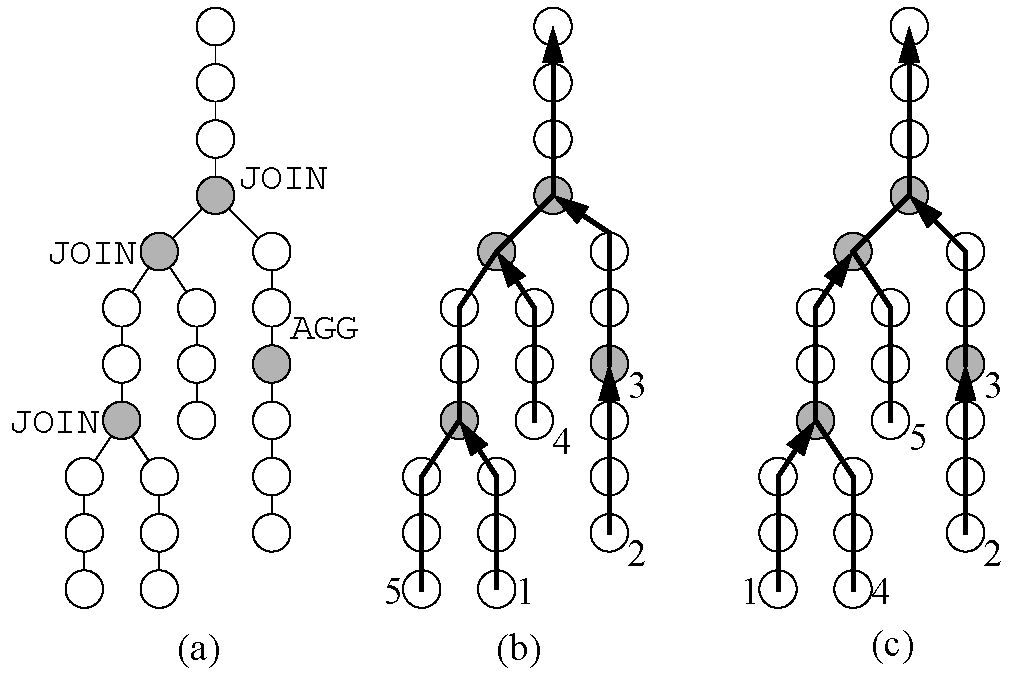
\includegraphics[width=6in]{DAG}
  \end{center}
\vspace{-10 pt}
  \caption{TCAP code containing three joins and an aggregation represented as a graph (a).  During physical planning, it must be broken into pipelines; two
potential pipelinings are shown in (b) and (c).}
  \label{fig:TCAP}
\end{figure}


\section{Pipelined Execution Details}
\label{sec:pipelined}

This section describes some of the details regarding PC's pipelined execution engine.  We begin by considering how a TCAP
program is used to build a set of pipelines, and then focus on interaction between pipelined execution and the PC object model
and memory management. The description in this section is mainly focused on a
single-thread scenario. We will introduce parallel and distributed
processing in Sec~\ref{sec:implementation}.

\vspace{5 pt}
\noindent
\textbf{Breaking a TCAP DAG into Individual Pipelines.}
The previous section discussed the problem of logical optimization for TCAP programs---optimization that takes into account the semantics
of the various operations, but does not consider actual implementation.  
Executing a TCAP program using PC's vectorized execution engine requires phyical planning as well.  The single most important physical 
optimization involves choosing how to break a TCAP program into a set of individual \emph{pipelines}, and then choosing an execution order
for those pipelines.
A pipeline is a list of TCAP operations that are executed in sequence over a vector list, with each operation performing some
transformation over the vector list; at all times as the vector list is pushed through the pipeline, it remains buffered in RAM.  
At the end of a pipeline is a \emph{pipe sink}, where one or more of the
vectors in a vector list is written out to a PC \texttt{Object}
container located on an output page, for later use (which may require shuffling or broadcasting the container across a PC cluster).  
For example, the pipe sink associated with aggregation
writes a vector of key \texttt{Object}s and a vector of value \texttt{Object}s to a PC \texttt{Map}, performing pre-aggregation when
applicable.
Each pipeline ends in a pipe sink, though only a few TCAP operations require pipe sinks: \texttt{JOIN} (where either one or both inputs are pipe
sinks, depending upon the join algorithm chosen), \texttt{AGG}, and
\texttt{OUTPUT}. In our current implementation, if one operation's
output has multiple consumers (the output is the input of more than one operations), the output will also be
materialized to a pipe sink.
Two different decompositions of a TCAP program into individual pipelines are shown in Figure \ref{fig:TCAP}.



\vspace{5 pt}
\noindent
\textbf{Ensuring In-Place Data Allocation of Output Data.}
Our primary goal when designing PC's pipelined execution engine is reducing  
memory-related costs.  
Since we 
encourage programmers to manipulate (potentially complex) PC \texttt{Object}s
rather than flat data, care must be taken to ensure that memory-related costs do
not dominate execution times.

Of all memory-related issues,  
data placement is paramount.  Because PC is designed to operate over
complex objects, data movement can be 
expensive.  To maintain the principle of
zero-cost data movement, \texttt{Handle}s pointing to out-of-block data are not allowed in PC.
Thus, copying a PC \texttt{Handle} from one memory block to another requires a deep copy of the target of the \texttt{Handle} to the new block.  
And since a
\texttt{Handle} may be declared as pointing to a super-type of its
target type (for example, an \texttt{Emp} object may be pointed to by a \texttt{Handle <Object>}), the correct code for invoking the deep copy of the
target must be executed via a virtual 
function call, which can in turn set off a cascade of virtual function calls. It is this chain reaction that we seek to avoid at all costs.
Thus, the most important principle governing the 
design of PC's pipelined execution engine is that \emph{data should be constructed where it is ultimately needed}.

To facilitate this, we note that user-supplied code will typically accept input data, then somehow use that input data to
create an output object.  For example, consider 
the following lambda term construction function, specifying the creation of output data:

\begin{codesmall}
Lambda <Handle <Emp>> getProjection (Handle <Sup> arg) {
        return makeLambda (arg, [] (Handle <Sup> &input) -> Handle <Emp> {
		return makeObject <Emp> (input->getName (), input->getDept ());
	});}
\end{codesmall}

\noindent
When the code corresponding to this lambda term is executed as a pipeline,
we wish to ensure that there is no need to move the \texttt{Emp} object created within the native C++ lambda to an output page.
To guarantee this,
PC obtains from the buffer pool a page for writing output objects for each thread, and places the current object allocation block
onto this page. 
When the call to \texttt{makeObject} within the lambda is executed, it will create the output \texttt{Emp} object
directly on the output page.  Any allocations triggered by the construction of the \texttt{Emp} will also be directly on the output page.

\vspace{5 pt}
\noindent
\textbf{Avoiding Unwanted In-Place Allocations.}
It is just as important to avoid unwanted allocations on an output page.  Depending upon the user-supplied
allocation policy, such allocations will either result
in holes on the page when it is shipped into the cloud and hence a lower data density (if no-reuse is specified), 
or else they will result in the utilization of CPU cycles to 
reclaim and reuse the memory. 

Some of the burden of avoiding unwanted allocations is placed on a PC programmer. A programmer should
avoid unnecessary calls to \texttt{makeObject ()}, specifically avoiding those calls that allocate data that can never possibly make it to an output object.

Likewise, the system should do the same.  It is most critical that PC avoid moving intermediate data to an output page during pipeline execution.
Reconsider the example of Section \ref{sec:vectorized}.  The user-specified \texttt{getSelection ()} describes
a computation that invokes \texttt{Emp::getDeptName ()}, checking whether it equals the extracted value of
\texttt{Dep::deptName}.  During pipelined execution, care is taken \emph{not} to store these intermediate results
on the output page.  The vector that results from extracting
\texttt{Dep::deptName} from each input object is allocated outside of
the output page, and stores C-style pointers to each \texttt{Dep::dept
  Name}
value that are simply dereferenced when the vector is used by subsequent pipeline stages.  
If \texttt{getDept Name ()} returns a reference, its output is treated similarly.  If 
\texttt{getDeptName ()} returns actual data (and not a reference), then that data is stored in a vector \emph{outside}
of the output page.  Thus, in the case that the returned object has \texttt{Handle}s that refer back to the input data, a deep
copy will not be invoked because those \texttt{Handle}s will physically reside on a memory location outside of the current
allocation block (as described previously, deep copies of the target of a \texttt{Handle}
happen only when a \texttt{Handle} is copied to the current allocation block).  
It is only when/if a subsequent operation copies the result (and the \texttt{Handle}s are contained)
to the output page (corresponding to the current allocation block)
that a deep copy happens.  Thus, intermediate data are \emph{lazily copied} to 
the output page, once \texttt{Handle} to the data is copied to the output page, which tends to avoid un-necessary allocations.

\vspace{5 pt}
\noindent
\textbf{Memory Dependencies During Pipelined Processing.}
All data produced via calls to \texttt{makeObject} are written to
allocation blocks housed on in-memory pages served to PC by the buffer
pool.  PC's pipelined
processing induces four types of pages, each of which has a different lifetime during which it must be buffered in RAM:

\begin{enumerate}

\item The first page type is an \emph{input page} that store the base data that will be processed by the pipeline.
To push vector lists into a pipeline, PC first loads a page containing a PC container (such as a PC \texttt{Vector}) of 
input data from the buffer pool, and then repeatedly creates vectors of \texttt{Handle}s to the objects on
the the page (the little `v' is intentional; these vectors are \emph{not} PC \texttt{Object}s themselves, as we do not want them to be allocated
on the current  allocation block, as they store only intermediate data).  PC wraps
each vector produced in a vector list, and sends the vector list into the pipeline.  This process is repeated until the input page is consumed.
The input page must be buffered as long as a vector list originally created using its data is making its way through the pipeline.  

\item A \emph{live output page} that houses the current allocation block.  All allocations happen on this block, and so this page may hold intermediate data
and/or output data.
Intermediate data are 
reachable only by vectors that have been produced
by non-sink stages in the pipeline; as described above, the expectation is that intermediate data will eventually become output data stored on the
same page, avoiding a copy.  Output data are
data written by the sink (terminal) node in the pipeline to a PC container 
\texttt{Object} (such as a \texttt{Vector} or a \texttt{Map} if the pipeline is feeding a join) that holds the ultimate output
of the pipeline.

\item Zero or one \emph{zombie output pages} that are full and store output data, but must
be pinned in RAM because they also store intermediate data.  This may happen when one or more vector lists make it all the way through the pipeline,
causing output data to be written by 
the sink node at the end of the pipeline.  Then, the next vector list only makes it part way through the pipeline before the live
output page
fills and an out-of-memory fault occurs.  
At this point, a new live output page is obtained for use
as the current allocation block.  However, since the previous live output page still contains valid intermediate data, it cannot be written out.  This 
page becomes a \emph{zombie output page} and remains that way until it cannot possibly hold any intermediate data, at which point it can be flushed.

Note that there can be at most \emph{two} zombie output pages for a pipeline,
because a pipeline is restricted 
to have just one sink.  
When a zombie output page is created, the vector list whose processing is
responsible for its creation may create references to intermediate data allocated to the new, live output page, and then processing of that
vector list begins
to fill the live output page with output data.  This may induce a second
out-of-memory fault, creating a second zombie output page.  However, since the vector list whose processing induced the fault is being
processed by the pipeline's sink, \emph{it cannot be used to produce additional intermediate data whose references will be held by the vector list} 
and can only produce output data.  Thus, any additional pages it is used to produce
cannot contain a mix of output and intermediate data.  Further, note that once a vector list makes it all the way through the pipeline, all of its references
to data are destroyed, so no pages can possibly
store valid intermediate data and hence all zombie output pages can be flushed---and hence the number of zombie output pages is capped at two.

\item Finally, there are zero or more 
\emph{zombie pages} that store only intermediate data.  These are similar to zombie output pages, but they do not store any output data; they
store only intermediate data.  Just like zombie output pages, all zombie pages can be flushed whenever a vector list is completely processed by a pipeline.
However, unlike zombie output pages, zombie pages should not be written back.
\end{enumerate}
